\documentclass[10pt,twocolumn]{article}

% \frenchspacing
% \setlength\parindent{0pt}

\usepackage[english]{babel}
\usepackage[stretch=10, shrink=10]{microtype}
\usepackage[a4paper, total={6.5in, 9in}]{geometry}
\usepackage{graphicx}
\usepackage{caption}
\usepackage{subcaption}
\usepackage{amsmath}
\usepackage{multirow}
\usepackage{xcolor}
\usepackage{hyperref}
\usepackage{float}

% Better vspace in enumerate/itemize
\usepackage{enumitem}
\setlist{noitemsep,topsep=0pt,parsep=0pt,partopsep=0pt}

% \setlength{\columnsep}{8mm}

\title{\textbf{Real-time guitar transcription using\\Fourier transform based methods}\\A pitch estimation framework and overtone sieve algorithm}
\author{Luc de Jonckheere}
% \date{}

\begin{document}
\selectlanguage{english}

\maketitle
%\tableofcontents


\section*{Abstract}
In this paper, we explore real-time transcription of a electric guitar signal. Data driven methods are not fast enough for real-time use, so we focus on Fourier transform based methods. We will provide a basis for monophonic transcription and a proof-of-concept algorithm for polyphonic transcription. The goal of this paper is to give an overview of the problems when trying to solve this problem and to provide an implementation in which different methods can be tested.
% In the field of automatic music transcription (AMT), data driven methods such as artificial intelligence and machine learning are becoming more popular by the year. This is especially true for multi-pitch estimation (also known as multiple $f_0$ estimation). Even though the results are getting better every year, little understanding of the problem is gained. The few papers which use mathematical models to solve this problem, do not publish their code which makes it difficult to build upon.

% In this paper, we will present an extensible pitch estimation system along with a harmonic sieve algorithm which can perform basic multi-pitch estimation. This system can be used as basis for further research of the individual components.


\section{Introduction}
Automatic Music Transcription (AMT) is a field of study which tries to convert acoustic recordings into some form of (digital) music notation~\cite{survey1}. This task can be divided into two subproblems: pitch estimation and onset detection~\cite{survey2}. Instead of trying to convert a song into music notation, this paper will focus on translating a guitar signal into a set of played notes in real-time. This problem is very similar to AMT, as both require pitch estimation and onset/offset detection, however, we also have take latency into account.

Single pitch estimation can be accurately performed using simple mathematical models~\cite{mono}. Multi pitch estimation is much harder as harmonic overtones are difficult to differentiate from the fundamental frequency~\cite{oud}. Because of this, most recent methods use machine learning or artificial intelligence. These methods are not well suited for real-time transcription. Also, no actual (mathematical) understanding of the problem is gained. Because of this, this paper will focus on mathematically solving this problem. Even if the methods researched in this paper might not outperform ML/AI solutions by themselves, they could be used to filter the input data for the ML/AI approaches. This might in turn improve the results of the AI/ML methods significantly.

Pitch estimation can be divided into a few subproblems. If a paper focusses on one of these subproblems, it also has to solve the other subproblems in order to test the system. Most papers do not publish their source code, which makes building upon other's work difficult. It also limits the research of the interaction between different solutions for the different subproblems. Because of this, we provide a framework in which can be built upon, as the implementation of a subproblem can easily be interchanged with another. The code can be found at "\url{github.com/lucmans/dechord}".

The goal of this paper is to give an overview of the problems when trying to solve this problem. This is done by developing a program which can translate a guitar signal to a set of observed notes in real-time. We also provide an algorithm which can estimate a set of played notes using the set of observed notes. The code should be publically available and easily extensible so others can optimize a subproblem without having to solve the other subproblems.

Note that this paper is a preliminary paper for a possible master thesis. The focus is on building a prototype which can perform monophonic AMT and presenting a first draft of a polyphonic version. Using this information, we will estimate if the thesis project is feasible.


\section{Related work}
Spectral peak picking based AMT methods are often deemed infeasible for real-time AMT~\cite{hater}, due to the relatively low resolution in the low frequencies when using the Fourier transform~\cite{theoretisch}. This problem cannot be alleviated by zero-padding the Fourier transform input, as it does not add any information, it merely increases the resolution by interpolation~\cite{infomax}\cite{infomax2} and increases the computing time of the transform~\cite{boek}. However, using quadratic interpolation, we can very accurately interpolate peaks within Fourier frequency bins~\cite{interpol}. Also, other transforms such as the constant Q transform~\cite{cqt} which do provide more resolution in lower frequencies are getting more popular, which will allow us to differentiate two notes on a very small interval.

A big problem in polyphonic pitch estimation is the occurrence of overtones~\cite{oud}. As these overtones also have a periodic nature in the frequency domain, they can be detected using another Fourier transform~\cite{double}. This does however have a big impact on the latency, as performing a Fourier transform is computationally expensive. Also, notes which are at octave intervals have the same periodicity~\cite{octave}, which makes them difficult to distinguish.

Another problem is choosing the real-time constraint for processing the input. Some papers claim 140 ms is sufficient~\cite{sloomboi}. This is however ridiculously long, as it would be about a note difference when playing eight notes in 200 BPM. Also, there already is a large latency due to how audio drivers work~\cite{os}. In practice, musicians often tweak their audio driver settings in order to gain 5 to 10 ms in latency, which makes the difference between being able to play faster pieces or not.

When limiting ourselves to transcribing a guitar, we can use physical limitations of the instrument to our advantage~\cite{physical}. However, this forces the guitarist to use the guitar in a specific way. For instance, these methods fail when the strings are tuned to different notes.


\section{Preliminaries}
In this paper, we use the Fourier transform to obtain a frequency domain representation of a signal. This transform takes a frame full of samples and produces a list of amplitudes corresponding to frequency bins. How this is done is described in Section~\ref{sub:four}.

When playing a note on an instrument, multiple frequencies are produced. The most notable is the fundamental frequency. Every note corresponds to one fundamental frequency. For instance, the fundamental frequency of the $\text{A}_4$ is 440 Hz. Integers multiples of the fundamental frequency resonate and produce harmonic overtones~\cite{overtones}. They are called harmonic overtones, as they are exact integer multiples and do not produce destructive interference among each other. Every integer multiple resonates with the fundamental frequency, however, each subsequent overtone is of lower amplitude.

Instruments do not produce perfect sine waves. The specific distortion of an instrument is called its timbre~\cite{timbre}. These distortions also show in the frequency domain. These are however very small compared to the fundamental frequency and its overtones of a note and can be disregarded as noise.


\section{Pitch estimation}
Automatic music transcription can be separated into two main problems; onset detection and pitch estimation~\cite{survey2}. In this paper, we will focus on pitch estimation. Because we always output the set of played notes for the last analysed frame, we do not require onset information. However, this information can improve the results of pitch estimation. For example, when an onset is detected, we can discard all samples from the transient.

As stated before, our goal is to perform the transcription in real-time. We choose a constraint of 6 ms. Most musicians work with a driver latency of 9 to 11 ms. On a good computer, this latency can be reduced to 3-5 ms. We will use these 6 ms of latency difference to perform our calculations in. Note that when playing more notes per second, latency becomes more of a problem. On slower pieces, we can get away with much larger latencies. In order to test the impact of extra latency for yourself, we developed a tool which plays back the incoming audio signal with a user specifiable delay. This tool can be found under the "latency" branch in our GitHub repository. Note that this tool adds a latency on top of the audio driver latency like our program would. The total latency is much larger than the displayed latency.

Pitch detection can be broken down into a few subproblems. First, a frequency domain representation of the signal is obtained (e.g. Fourier transform). Then, significant peaks have to be selected from the frequency domain. Based on the found peaks, we have to determine what notes were actually played on the instrument.

\subsection{Transform to frequency domain}
To estimate the frequency components of a frame, transforms are used. Most commonly, the Fourier transform is used as it is the most researched transform and much is known about it~\cite{survey2}. Its main downside is that the frequency bins are constant in size, where the distance between notes increases exponentially. Because of this, low notes are hard to discern in the frequency domain where high notes have more resolution than needed. Because of this, other transforms such as the constant Q transform (CQT) are getting more popular.

When using transforms, window functions have to by applied to the frames to prevent spectral leakage~\cite{window}. Furthermore, the actual peak locations can be accurately interpolated using (Lagrangian) quadratic interpolation~\cite{interpol}. These concepts are further described in Section~\ref{sub:four} and Section~\ref{sub:peak} respectively.

\subsection{Peak picking}
Peaks in the frequency domain correspond to predominant frequencies in the analysed frame. However, not every peak is of interest. Some peaks are generated by noise. Many of these peaks can be filtered by requiring a minimal signal level to be considered a peak. Furthermore, due to spectral leakage, peaks can be observed which are not in the original signal. This kind of noise can be minimized by choose a good window function~\cite{window}. In polyphonic signals, harmonic overtones of different notes may interfere, which will may lead to inconsistent and oscillating peaks.  % TODO: Maybe make preliminary section about overtone dissonance

On order to determine if a peak is significant enough, we first calculate a Gaussian average envelope~\cite{gauss}. For every point in a frame, the Gaussian average is a weighted average of all points in the frame. The weight is determined by the distance from the current point. The distance in number of bins goes through a Gaussian function to determine the actual weight. Here, higher values for $\sigma$ make points close by weight more compared to distant points. How this envelope is precisely calculated and used for peak picking is described in Section~\ref{sub:peak}.

\subsection{Note sets}
Given the spectral peaks from the previous step, we can try to calculate what notes they represent. Unfortunately, the found peaks do not only contain fundamental frequencies, but also harmonic overtones. This is only a small problem in monophonic transcription, as there is only one fundamental frequency and its overtones. However, in the polyphonic case, it is difficult to determine which peaks are fundamentals and by extension know how many notes are played at the same time.

To determine if notes are fundamentals or overtones, we use a "harmonic overtone sieve". Here, we look if any higher peak can be explained by the currently considered peak. The more other peaks a peak can explain, the more likely it is to be a fundamental. Moreover, if we cannot explain a certain peak, it is likely that there is a second note in the source signal.


\section{Implementation}  \label{sec:impl}
The program developed for this paper is written in C++ (11) and compiled with g++ (10.2.0). It uses SDL (2.0.14) for audio input/output and spectrum visualisation. FFTW (3.3.9) is used for efficient Fourier transforms. Its code can be found at "\url{github.com/lucmans/dechord}".

There are many parameters which change the behaviour of the overall system. For this paper, we choose some values which seemed to perform well. The values can still be optimized for better results. All parameters can be found in \texttt{config.h} along with comments explaining them.

By default, the program assumes an $A_4$ of 440 Hz. This can also be edited in \texttt{config.h}. Only 12 tone equal temperament (12-TET) tuning is currently supported. It could easily be changed to n-TET tuning, but non TET tuning is not easily supported.

\subsection{Transform to frequency domain}  \label{sub:four}
Our program uses the Fourier transform to obtain the frequency domain representation. We choose this transform as FFTW provides a very fast implementation. This speed is necessary for the real-time constrains on our system.

The resolution of the Fourier transform is dependent on the number of samples in a frame. We sample the guitar signal at 192 kHz, which is the maximum sample rate for most audio interfaces. To allow guitarists to play mildly fast, we have to limit our frame length. If the frame size if too large, multiple separate notes may be included in one transform, which would make it seem like the notes were played at the same time. Moreover, frame sizes which are a power of two can be transformed more efficiently, which further restricts are frame size choice. We chose a frame size of $2^{14} = 16384$ samples, which at 192 kHz is 0.085 seconds (11.72 frames per second). This gives us a Fourier bin size of 11.72 Hz. At first glance, such a large bin size seems like a big problem, as the smallest interval that can be played on a guitar (G\#\textsubscript{2}-A\textsubscript{2}) is about 6 Hz. However, the overtones of these notes will have more Hz between them, which makes to possible to differentiate the two notes.% Also, as discussed in Section~\ref{sec:future}, we might be able to increase the frame size without reducing our frame rate too much.

Before applying the transform, a window function is often applied to minimize the artifacts produced by the transform. In this paper, we mainly use the Blackman-Nuttall window, but the following windows are also provided: Hamming window, Hann window, Blackman window, Nuttall window, Blackman-Harris window, Flat top window. Other window functions can easily be added.

\subsection{Peak picking} \label{sub:peak}
Three different peak picking algorithms have been implemented. The first picks every local maximum (every \texttt{i} where \texttt{data[i - 1] < data[i] \&\& data[i] > data[i + 1]}). This approach finds too many peaks, especially in noise. The other two algorithms pick peaks based on a Gaussian average envelope. One algorithm picks all peaks which are above this average and the other only picks the highest peak for each spectral lobe above this average. Only picking the highest peak seemed to restrictive in testing, however, it is better resilient against noise and may be used with more careful parameter optimisation. By using the envelope, we effectively filter small local maxima close to large local maxima.

The Gaussian average envelope is calculated for every Fourier bin $i$ by taking the weighted average of a arbitrary number of bins around $i$. The weights are determined by a Gaussian function ($e^{-\pi(\frac{x}{\sigma})^2}$). The value of $\sigma$ and number of bins around $i$ can be changed in \texttt{config.h}. Higher values for $\sigma$ makes points around the considered point have a higher weighting. In our implementation, $\sigma$ is set to 1.2 and the number of bins is set to 47.

Even though this envelope works well for parts of the spectrum with peaks, it will still find peaks in noisy areas without peaks. This can be prevented in two ways. The first is setting a threshold which a peak has to exceed. This will result in less sustain, but works well. Secondly, we know that peaks outside the frequency range of a guitar cannot be a fundamental frequency. We can discard peaks lower than the lowest note, but peaks higher than the highest note still provide us information as it might be an overtone.

It is possible to determine the actual peak location within a Fourier bin using quadratic interpolation~\cite{interpol2}. Here, we calculate a value $p \in [-\frac{1}{2}, \frac{1}{2}]$, which is the location of the actual peak relative to the found peak in number of Fourier bins. In order to calculate $p$, we need the height of our found peak ($y(0)$) and the height of the two neighbouring bins ($y(-1)$ and $y(1)$). As quadratic interpolation is more accurate in the dB (logarithmic) scale, we define:
\begin{center}\vspace{-1mm}
    $\alpha = \log y(-1)$\\
    $\beta = \log y(0)$\\
    $\gamma = \log y(1)$
\end{center}\vspace{-1mm}
Then, we can calculate $p$ as follows:
\begin{center}\vspace{-1mm}
    $p = \frac{1}{2} \frac{\alpha - \gamma}{\alpha - 2\beta + \gamma}$
\end{center}\vspace{-1mm}
Given the Fourier bin size, we can calculate the frequency of the peak $i$ by multiplying the bin size by $i + p$.

\subsection{Note sets}  \label{sub:impnoteset}
Using all the found peaks, we can determine which peaks are overtones and which are fundamentals. First, we determine which notes the frequencies represent and calculate the error on these notes. The error is calculated as the number of cents from the closest harmonic note. The errors are different for every overtone (the series of errors is constant for every harmonic overtone series), as overtones are dissonant compared to equal temperament tuning. See Table~\ref{tab:overseries} for an example.
\begin{table}[H]\vspace{-3mm}
    \centering
    \begin{tabular}{rrcrr}
        $n$ & $f_{\text{overtone}}$ & closest note & $f_\text{note}$ & error \\
        \hline
        0 & 261.626  & $C_4$    & 261.626  &  0 \\
        1 & 523.251  & $C_5$    & 523.251  &  0 \\
        2 & 784.877  & $G_5$    & 783.991  &  1.955 \\
        3 & 1046.502 & $C_6$    & 1046.502 &  0 \\
        4 & 1308.128 & $E_6$    & 1318.510 &  -13.686 \\
        5 & 1569.753 & $G_6$    & 1567.982 &  1.955 \\
        6 & 1831.379 & $A^\#_6$ & 1864.655 &  -31.174 \\
    \end{tabular}
    \caption{Example of overtone series and the errors compared to the closest note}
    \label{tab:overseries}
\end{table}\vspace{-3mm}
If only harmonic notes were played on a guitar, we could filter all notes with an error higher than an arbitrary threshold. However, as most guitars are not perfectly intonated and strings detune by pressing them down on a fret, this information has to be used with care. Correctly using this information is out of the scope of this paper.

Creating a monophonic algorithm is relatively easy given the frequencies of the peaks. For instance, we can iterate over all found peaks and check if every higher peak can be a overtone of the considered peak. After counting the number of overtones for every peak, we can pick the peak with the most overtones.

Due to small errors, the overtones are not exactly integer multiples of the fundamental. As the distance between notes increases with frequency, we cannot set a constant threshold of error in Hz. Instead, we calculate the error in cents and choose a threshold for this error (configurable in \texttt{config.h}). This also allows for equal error tolerance above and below the note, which percentage based methods would not.

Polyphonic note detection can use a algorithm similar to the monophonic algorithm. As the number of played notes in unknown in the polyphonic case, we have to determine if a note is a fundamental or overtone. We cannot just set a threshold for the number of overtones a fundamental should have, because the number of detected overtones is very inconsistent. To solve this, we present a harmonic overtone sieve algorithm. Instead of directly looking for fundamentals, we try to sieve away all harmonics until we are left with fundamentals. We start at the lowest peak end mark all its possible overtones. If there are still unmarked peaks left, they are likely from another note and we sieve its overtones away. We can repeat this process until no more peaks can be sieved. If two peaks are not distinguishable in the root notes but are in the overtones, this algorithm will report the first distinguishable overtone as the root note. It is possible to calculate what the root note should have been, but that is outside the scope of this paper and will be further discussed in Section~\ref{sec:future}.

After this, we can remove all peaks which are outside of the frequency range of a guitar. The minimum and maximum can be changed in \texttt{config.h} to accommodate for different tunings of guitars with extra strings.

\subsection{Latency}
The latency of our system can be divided in two different latencies, the time to fill a frame with samples and frame processing time. Because our algorithm works on a "per frame" basis instead of a "per sample" basis, we have to wait until the audio driver has fetched enough samples for us to fill a frame. The time it takes to start analysing a frame after receiving the first sample of this frame can be calculated by dividing the number of samples per frame by the sample rate. This is equal to the length of a frame. In practical terms, it is the maximum latency on detecting a newly played note. The average latency is obtained by dividing this number by two.

We use a frame size of 16384 samples and a sample rate of 192000 samples per second, which equates to a frame length of 85.3 ms. This is well over our real-time constraint. Unfortunately, we cannot change this value too much. The sample rate is already at the maximum of most audio interfaces. We also cannot lower the number of samples per frame while using the Fourier transform, as it would further reduce the frequency resolution. However, as will be explained in Section~\ref{sec:future}, this might not be a problem, as we can reduce this latency by using partially overlapping frames.

We can control the second kind of latency by optimizing our algorithms. In Section~\ref{sec:exp}, we will measure the processing time of the different algorithms.


\section{Experiments}  \label{sec:exp}
We will perform a few experiments to test our system. The used audio equipment has a large effect on the results and in turn effects what parameters work best for the system. During development, an electric guitar with active EMC humbucker pickups was used. To convert the analog signal to a sampled digital signal, a Behringer UMC404HD was used. This audio interface has a dynamic range of 100 dB. Like most audio interfaces, this is much less than the dynamic range of a sample (144 dB for 24 bit integer). We opted not to amplify the signal in software, as it will distort it; especially if not done carefully. The tests were performed on an AMD 3700X CPU.
%
% Often used datasets for evaluating pitch estimation focus on different goals than this paper. For instance, they focus on transcribing multiple instruments at once or having instrument invariance. They also do not focus on real-time transcription, which makes the problem much harder. However, in order to present some comparative measure, we will use the Mirex dataset for "Multiple Fundamental Frequency Estimation \& Tracking"~\cite{data}. TODO (when I receive it): Short description of dataset.

We constructed our own dataset to evaluate the performance. This dataset is a technical dataset consisting of scales and intervals played on a guitar. Scales allow us to measure the monophonic performance. As scales are easy to play, multiple recordings should have the same results. This allows us to isolate and measure other variables, such as the effect of tempo or playing the scale higher/lower. Recordings of different intervals allow us to measure the polyphonic performance. By measuring all two note intervals, we can identify any problems with specific intervals. As the distance in frequency in an interval increases when the same interval is played at higher notes, we record the intervals at multiple root notes. We will also measure the performance on the four basic triads: the major triad, minor triad, augmented triad and diminished triad.

Note that when repeating our experiments, your results may very slightly. This is because the results of the Fourier transform from FFTW are not consistent~\cite{fftw}. This is especially noticeable in inconsistent latencies.

\subsection{Monophonic performance: scales}
To test the monophonic performance of our system, we first measure the performance of scales at different pitch ranges. The scales are played at a speed of two notes per second. This equates to playing fourth notes on 120 BPM. We play the scales at a relatively slow speed, such that this cannot become a limiting factor. The slower speed also helps to see if mistakes are the result of transients, as these mistakes should vanish as the note persists. We only play the C major scale, but change the starting note (mode). We play the full vertical scale from this starting note~\cite{scale}. Each position has 17 notes, except for $\text{F}_2$, which has 18 notes. In Table~\ref{tab:monperf}, we summarize the results of the experiment. We denote the different starting positions as $n_\text{start}$. For every starting position, we denote the accuracy ($a$), the accuracy without transient errors ($a_\text{trans}$), the accuracy without octave errors $a_\text{oct}$ and the adjusted accuracy without both of these errors ($a_\text{adj}$). The accuracy is calculated by dividing the number of correctly determined frames by the total number of frames with notes. The only frames without notes are positioned at the start and end of a file. We omitted these frames from the results, as they are always correctly determined to be empty frames. Erroneous notes due to transients usually have a lower amplitude where octave errors usually have a higher amplitude compared the amplitude of the base note. This allows is to distinguish between them. This information cannot be used to detect transients in real-time, as we compare the amplitude of the erroneous note to amplitude of the correct note in the following frames.
\begin{table}[H]\vspace{-3mm}
    \centering
    \begin{tabular}{r|rrrr}
        $n_\text{start}$ & $a$ & $a_\text{trans}$ & $a_\text{oct}$ & $a_\text{adj}$ \\
        \hline
        $\text{E}_2$ & 91.4\% & 95.2\% & 96.2\% & 100\% \\
        $\text{F}_2$ & 92.3\% & 96.2\% & 96.2\% & 100\% \\
        $\text{G}_2$ & 92.0\% & 95.0\% & 97.0\% & 100\% \\
        $\text{A}_2$ & 93.0\% & 94.0\% & 99.0\% & 100\% \\
        $\text{B}_2$ & 92.8\% & 96.9\% & 95.9\% & 100\% \\
        $\text{C}_3$ & 92.8\% & 92.8\% & 100\%  & 100\% \\
        $\text{D}_3$ & 96.0\% & 98.0\% & 98.0\% & 100\% \\
        $\text{E}_3$ & 96.7\% & 96.7\% & 100\%  & 100\%
    \end{tabular}
    \caption{Accuracy of monophonic $f_0$ estimation on C major scale at two notes per second for different starting positions. $a_\text{trans}$ is the accuracy without transient errors and $a_\text{oct}$ is without octave errors. $a_\text{adj}$ is the accuracy without both of these errors.}
    \label{tab:monperf}
\end{table}\vspace{-3mm}
We can see that the transient errors occur about 96\% of the time. There are two outliers at $\text{C}_3$ and $\text{D}_3$, which are the cause of inconsistent quality the played scales. This shows us that the guitarist has to play carefully for the best results. Furthermore, we noticed that the first played note almost always had a transient error. This could be because we start playing from a silent signal instead of changing from a previous note. Also, the transient errors show up more often between lower frequency notes. Almost all octave errors are at note changes, so better transient filtering will also solve these cases. Other than these errors, the system seems to work perfectly.

\subsection{Polyphonic performance: intervals}
To test the polyphonic performance of our system, we let it determine the played notes in an interval. We play every interval within an octave to test if there are any problems with separating the notes in specific intervals. For instance, some interference may cause oscillating peaks in the frequency domain. Again, we try all the intervals at different root notes, as the pitch of the root note may make a big difference in performance. As we mentioned before, when two peaks are too close together, we cannot distinguish them. Often, the second note is distinguished an octave higher. We set the overtone error threshold to 10 cents. This is a relatively small value, but this allows us to see small problems in our algorithms better. Furthermore, as described in~\ref{sec:future}, we should not use a constant value, but use a different value for every $n$-th overtone. In Tables~\ref{tab:polperf1}--\ref{tab:polperf3} is a summary of the results. Here, we list the number of semitones $n$ between the two notes in an interval, if both notes were correctly found. If not, we denote if the second note was detected an octave higher. This often happens, because we cannot distinguish two notes in small intervals at low pitches. The last column shows if there were other notes reported which were not transients.
\begin{table}[H]%\vspace{-2mm}
    \centering
    \begin{tabular}{r|lll}
        $n$ & both & octave & other \\
        \hline
        1  & false & true & 1-3 slightly inharmonic overtones \\
        2  & false & false & - \\
        3  & false & true & $\text{C}_4$ and $\text{G}_4$ (+ random at start) \\
        4  & true & - & Sometimes octave instead\\ &&& and 1-2 inharmonics at start \\
        5  & true & - & 1 slightly inharmonic overtone \\
        6  & true & - & 1-3 slightly inharmonic overtones \\
        7  & true & - & no \\
        8  & true & - & no \\
        9  & true & - & occasional inharmonic overtone \\
        10 & true & - & 1-2 slightly inharmonic overtones \\
        11 & true & - & 1-2 slightly inharmonic overtones
    \end{tabular}
    \caption{Performance of distinguishing notes in an interval with root note $\text{A}_2$.}
    \label{tab:polperf1}
\end{table}
\vspace{-3mm}
\begin{table}[H]
    \centering
    \begin{tabular}{r|lll}
        $n$ & both & octave & other \\
        \hline
        1  & false & true & about 4 slightly inharmonic overtones \\
        2  & false & true & about 4 slightly inharmonic overtones \\
        3  & true & - & $\text{C\#}_6$ or $\text{E}_6$ in first few frames \\
        4  & true & - & no \\
        5  & true & - & no \\
        6  & true & - & no \\
        7  & true & - & $\text{E}_4$ often filtered \\
        8  & true & - & random note 3 times \\
        9  & true & - & no \\
        10 & true & - & no \\
        11 & true & - & no
    \end{tabular}
    \caption{Performance of distinguishing notes in an interval with root note $\text{A}_3$.}
    \label{tab:polperf2}
\end{table}
\vspace{-3mm}
\begin{table}[H]
    \centering
    \begin{tabular}{r|lll}
        $n$ & both & octave & other \\
        \hline
        1  & false & true & occasional $\text{E}_6$ \\
        2  & true & - & no \\
        3  & true & - & no \\
        4  & true & - & no \\
        5  & true & - & no \\
        6  & true & - & no \\
        7  & true & - & no \\
        8  & true & - & no \\
        9  & true & - & no \\
        10 & true & - & no \\
        11 & true & - & no
    \end{tabular}
    \caption{Performance of distinguishing notes in an interval with root note $\text{A}_4$.}
    \label{tab:polperf3}
\end{table}%\vspace{-3mm}
In the tables, we can see that the algorithm performs well on higher pitched intervals. On medium pitched intervals, the small intervals become more of a problem, but most intervals are detected correctly. Transients are however visible for longer in the small intervals. Big problems arise when we look at the lower pitched intervals. There is much noise in the results and many slightly inharmonic overtones are reported. These could be filtered out by increasing the overtone error threshold, but that does not solve the overtones being inharmonic. The inharmonic overtones are less of a problem for larger intervals.
%
% We also look at the percentage of overtones that is filtered throughout a recording of an interval.
% As the harmonic overtone sieve algorithm is only a proof of concept, absolute performance measurements will yield bad results. By measuring the performance relative to having no filtering, we can show the effectiveness of our algorithm. This is done by measuring the percentage of overtones that is filtered throughout a recording of an interval. TODO: See Figure~\ref{fig:relative} for some examples of 
%
% Lastly, we will measure the performance on the four main triads: the major triad, minor triad, augmented triad and diminished triad. TODO: Experiment

\subsection{Latency}  \label{sub:algspeed}
The processing time of our system is very important, as it will directly impact the latency. We will only measure the time between receiving a frame from the audio driver until the answer is computed, as the time spent waiting on enough samples is fully determined by the number of samples in a frame and the sampling rate. The total processing time and the processing time of the individual steps and the total system can be seen in Figure~\ref{fig:snel}. Here, we only measure the latency on frames which contain peaks.
\begin{figure}[t]%\vspace{-2mm}
    \centering
    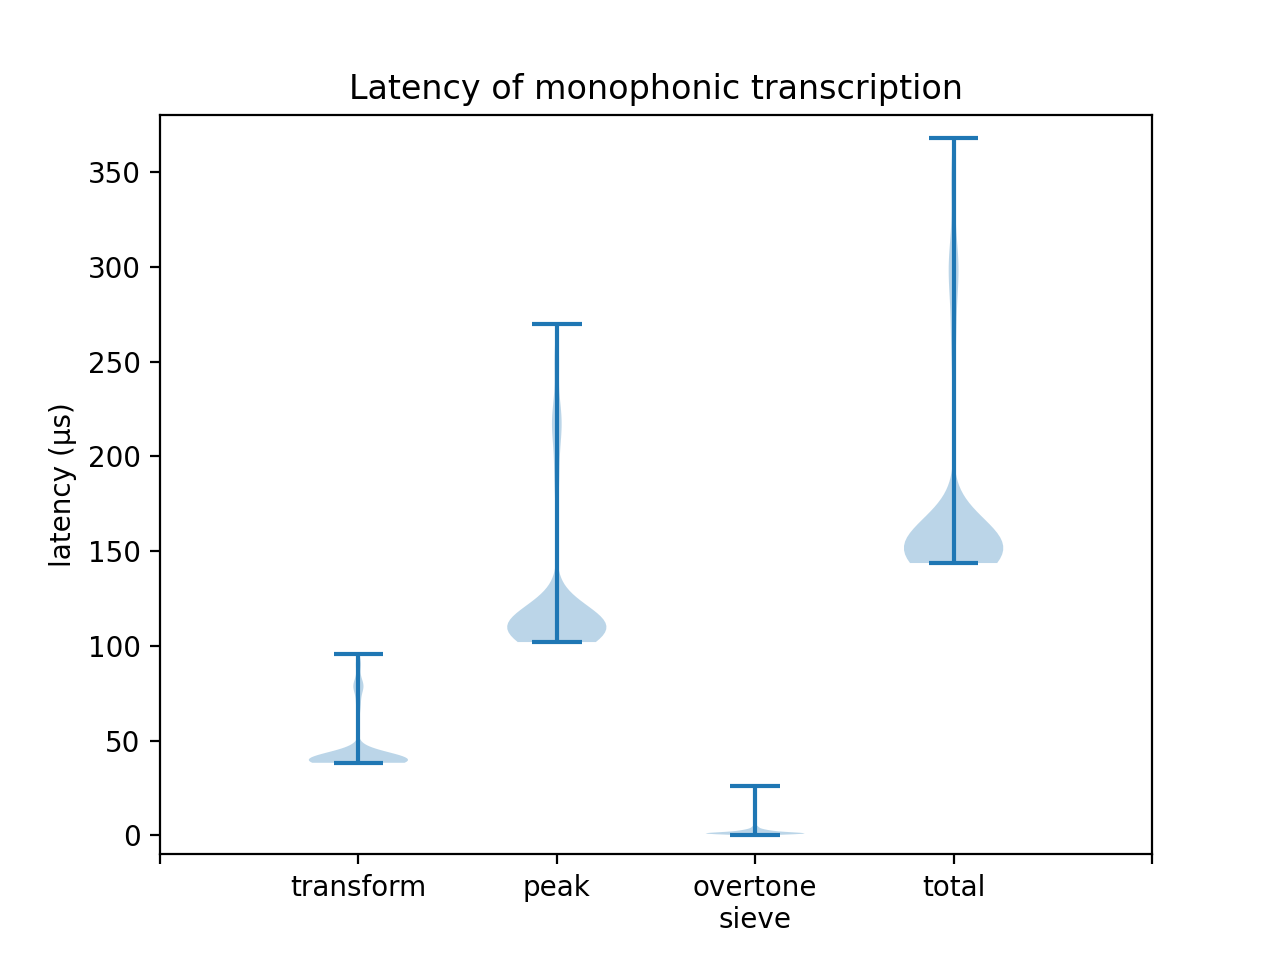
\includegraphics[width=\linewidth]{1.png}\vspace{+6mm} %0.85
    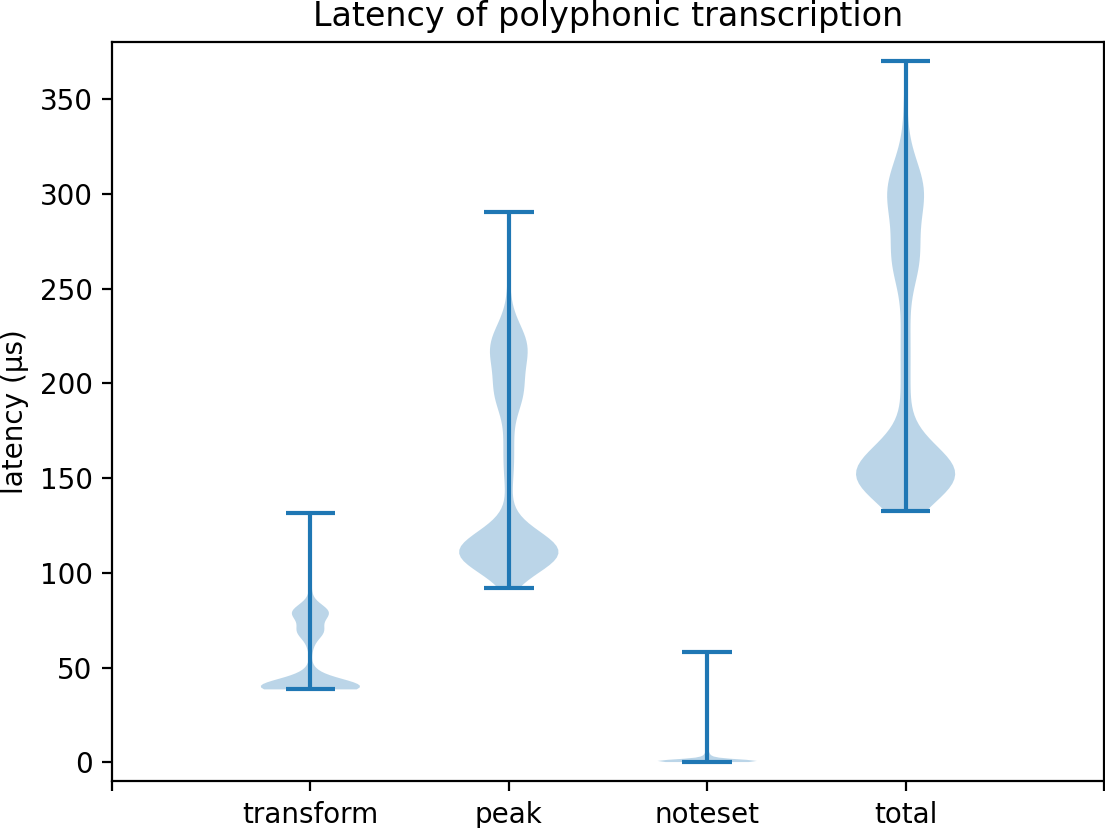
\includegraphics[width=\linewidth]{2.png} %0.85
    \caption{Processing time of the different algorithms}
    \label{fig:snel}
\end{figure}%\vspace{-4mm}
The total latency is never higher than 360 microseconds. In other words, we are at least 240 times real-time. This is well within out real-time constraint if we disregard the latency to fill a frame. Surprisingly, the peak picking algorithm is more compute intensive than the transform. Most of the time, the latency is on the lower end of the distribution. The outliers are mostly a result of transients. During transients, there are a lot more peaks to process, which slows down the different algorithms. This is especially the case for polyphonic transcription, as we have to take all the peaks into account. In the polyphonic dataset, transients contain more peaks as multiple strings are strummed. This results in a second lobe in the mid segment of the latency distribution.


\section{Conclusions}
In this paper, we presented and implemented a Fourier transform based AMT system and tested if these methods are feasible for real-time transcription. We divided the task in three components which can all be separately interchanged to facility specialized research in one of the components. The components are: obtaining the frequency domain representation, spectral peak picking and note selection. As shown in Section~\ref{sub:algspeed}, these tasks can be performed well within our real-time constraint of 6 ms. However, when using Fourier transform based methods, we need large frame sizes to get the required accuracy to discern lower pitched notes. Given the maximum sampling rate of widespread audio interfaces, it takes too long to fill a frame. The current implementation requires frame sizes of 16384 samples, which equates to frame lengths of 85 ms. As described in~\ref{sec:future}, we might still be able to use Fourier transform based methods for real-time transcription. However, other transforms such as CQT or wavelet transform might be better suited for real-time transcription, as we can still spare much compute time to lower the frame-wait time.

Even though we do not meet our real-time goal of 6 ms, we do have a high monophonic accuracy of 90\%. Almost all of the mistakes the cause of transients and fall between two notes. The other occasional mistake is an octave error, which is a difficult problem to solve. If we account for these two kinds of errors, our system has a 100\%. Our proof-of-concept harmonic sieve algorithm is capable of filtering many harmonic overtones and is able to distinguish between all intervals of more than 3 semitones. It is also able to isolate the two played notes on higher pitched intervals, however, there still is much noise on lower pitched intervals.

Our peak picking algorithm works fine for monophonic transcription, however, it does not work too well for polyphonic transcription. For instance, peaks in close distance to each other are easily missed. It is also compute intensive when compared to the other components and has the largest outliers. Even though the outlier are relatively very severe, they are all within 200 microseconds and might not be noticeable.

All code related to this project can be found at "\url{github.com/lucmans/dechord}".


\section{Future work}  \label{sec:future}
Our program serves as a good starting point for further research. However, there are still some problems with our current implementation. Solving these is outside of the scope of this paper and will be the topic of the follow-up thesis, but we will address the problems here. The first big problem is transients. They will appear as many random peaks in the frequency domain. Many of these peaks will be outside of the fundamental frequency range of a guitar, but not all of them, so discarding all high peaks does not solve the problem. Usually, during transients, there any significantly more peaks and even multiple peaks within one note. If this can pattern can consistently be detected, samples can be discarded until the transient is filtered.

The Fourier transform requires too many samples in a frame to remain within the real-time constraint while still providing the necessary frequency resolution in the fundamental frequencies. It might be possible to alleviate this problem with other transforms, such as the constant-Q transform or the wavelet transform, but those transforms may have to solve other problems. As mentioned before, the low resolution does not have to be a problem, as less resolution is needed when discerning higher pitched peaks. Currently, we do not detect enough overtones, but some testing showed us we can detect many overtones if we amplify the signal. This has to be done carefully, as artifacts may be introduced in the signal. Optimally amplifying of a recording is trivial, however, it is trickier in real-time. Using amplified signals would require recalibration of the peak picking parameters or even require a new algorithm in general.

The current implementation has no onset detection. We stated before that onset detection may help to filter out transients. If we can detect the transient in the time domain, we can discard all samples containing the transient. This may however be very difficult to do in real-time. If we can detect that there was a transient in a transformed frame, we are too late to act on it due to the large frame times. We can circumvent this by transforming partially overlapping frames. This could be done in different threads to limit the extra computational pressure which could impact our latency. However, as we are about 240 times real-time, we could likely perform it single threaded. Now, if we have a bad frame, we have to wait a full frame (83 ms) for the next estimation. However, if we use $n$ partially overlapping frames, we can try another estimation in $83/n$ ms. This will increase the responsiveness of our system greatly.

It is virtually impossible to know on what string a certain note was played. Furthermore, when playing an octave, the overtones of the lower pitched note align perfectly with the higher note and its overtones. If the strings were deliberately detuned to orthogonal frequencies, we can easily distinguish between the played strings. This does however create more peaks in the frequency domain. This tradeoff is worth further research.



\addcontentsline{toc}{chapter}{Bibliography}
\bibliographystyle{plain}
\bibliography{paper}

\end{document}
 